% Descrivere l'area utilizzata con foto di area con sovrapposta area suitable, differenza tra area dei tetti e area suitable per far notare come non sia fatto a caso. Quanta della suiatable are è stat utilizzata per il deployment. Andamento roi per i diversi valori della threshoold. Paragone classic vs greedyq3

%Fare foto con differenza di treshold da satellite,
% vedere se si riece a calcolare quanto si sovrappongono le soluzioni optimal vs classical
%Figura 2 trovare tetto con percentile che non fuoriesce

\subsection{Suitable area identification and optimization}
We tested the proposed framework on a district of  \omitted{the city of Turin} represented in Figure \ref{fig:satellite}. The satellite view of the area used for the test is overlapped with the result of step \ref{subsec:suitablearea}: the green area represents the total surface of the roofs (around $1,700,000m^2$, i.e., $1.7km^2$), while the red area represents the area that is suitable for PV installation (about $8340m^2$). It is interesting to notice that just 0.5\% of the available roof surface is considered suitable for PV installation. \attenzione{This underlines that the DSM data management strategy followed in this work allows to optimize data memorization, as only few DSM points are used to filter the suitable area, and full irradiance traces are generated only for a very limited portion of the district.} %analysis like the one proposed by our framework are extremely important to maximize the value of the investment for an EA, and that the DSM data management strategy adopted in this work allows to optimize data memorization to cover a large area.} 
 
\subsection{Optimal placement setup}
In our setup, we consider a PV-MF165EB3 module by Mitsubishi \cite{datasheet} organized in strings of 8 PV modules. The algorithm is set to allow maximum distance among panels on the same series $maxD$ of 3 meters, and a maximum height difference $maxH$ in the same series of 0.5 meters. This configuration allows to place in the same series PV modules positioned on different but almost contiguous roofs. An example of this scenario is visible in the top of Figure \ref{fig:satellizeZoom}, \attenzione{where it can be noted that the left portion of the suitable area spans across two roofs.}
\begin{figure}[!htbp]
\centering
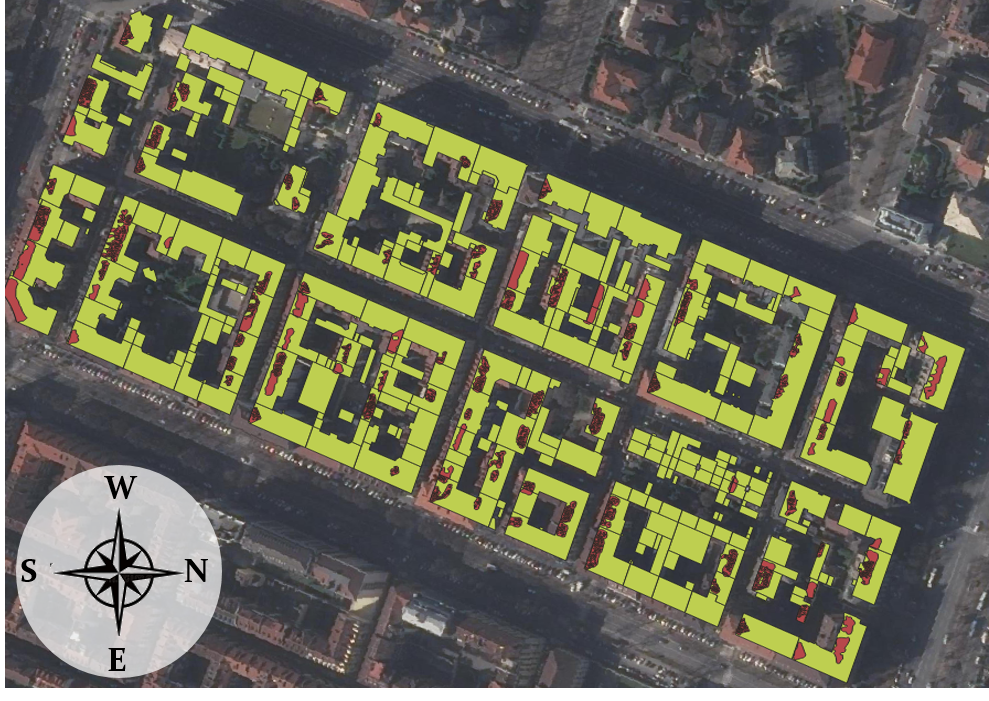
\includegraphics[width=\linewidth]{images/satellite3.png}\vspace{-0.4cm}
\caption{Satellite view of the area used for the test}
\label{fig:satellite}
\end{figure}

\subsection{Analysis of the identified PV placements}
%spiegare come si trasforma la suitable area per calcolare le tracce, tool utilizzati. menziorare il fatto che parto dal dsm identifico i tetti, per ogni tetto trovo la suitable area e trovo l'altezza e me la segno. Spiegare meglio il come si passa da dsm a tracce
To test the performance of the placement, we executed the algorithm multiple times with different values of $minTh$, i.e., the threshold of the 75-th percentile used to consider only the most promising portion of the suitable area. The results are reported in Table \ref{tab:areaused}. When increasing $minTh$, the area considered promising is reduced as a number of suitable locations are removed as featuring a 75th percentile lower than $minTh$. Thus, both the percentage of exploited area and the number of placed PV modules decrease when increasing $minTh$. 
% In Table \ref{tab:areaused} we can see how increasing $minTh$ involves a reduction of the amount of panels placed, as an effect of a reduction of the percentage of exploitation of the suitable area (as a lower portion of the roof has 75th percentile larger than $minTh$). 
An example is shown in Figure \ref{fig:satellizeZoom}: when $minTh$ is set to 100, 21\% of the available surface is considered suitable for PV placement; when $minTh$ is increased to 500, only 2\% of the area is considered suitable for PV installation, and as a result far less PV modules (colored rectangles) are installed on the same portion of roof. %\attenzione{forse avrebbe più senso far vedere cosa succede con 100 e 400? così serve a poco}
If we plot the number of PV modules installed (top of Figure \ref{fig:production}), we can observe that the decrease is not linear w.r.t. the threshold: as an example, moving from 200 to 300 the number of panels (and the area exploited) are reduced by $2/3$, as a wide percentage of locations has 75th percentile between 200 and 299. %In the following subsections we will see the effect of this behaviour on the power production and on the payback time.
% \begin{tabular}{|p{2.5cm}|p{0.8cm}|p{1.2cm}|p{1.5cm}|}
%\hline
%\textbf{75-th percentile threshold ($minTh$)} & \textbf{\# of panels} &\textbf{Installation area  ($m^2$)} &\textbf{Suitable area used (\%)} \\
\begin{table}[!tbp]
%\resizebox{\linewidth}{!}{%
\caption{Percentage of area used by PV placement over the total suitable area when varying $minTh$ }
\label{tab:areaused}
\centering
\begin{tabular}{|r|r|r|r|}
\hline
\textbf{Threshold} & \textbf{Panels} &\textbf{Installation} &\textbf{Suitable area} \\
\textbf{($minTh$)} & \textbf{(\#)} &\textbf{area ($m^2$)} &\textbf{used (\%)}\\
\hline\hline
100 & 1,792 & 1,540 & 21 \\\hline
200 & 1,536 & 1,319 & 18 \\\hline
300 & 656 & 561 & 8 \\\hline
400 & 464 & 394 &6 \\\hline
500 & 176 & 148 & 2 \\\hline
\end{tabular}%
\end{table}

\begin{figure}[!tbp]
\centering
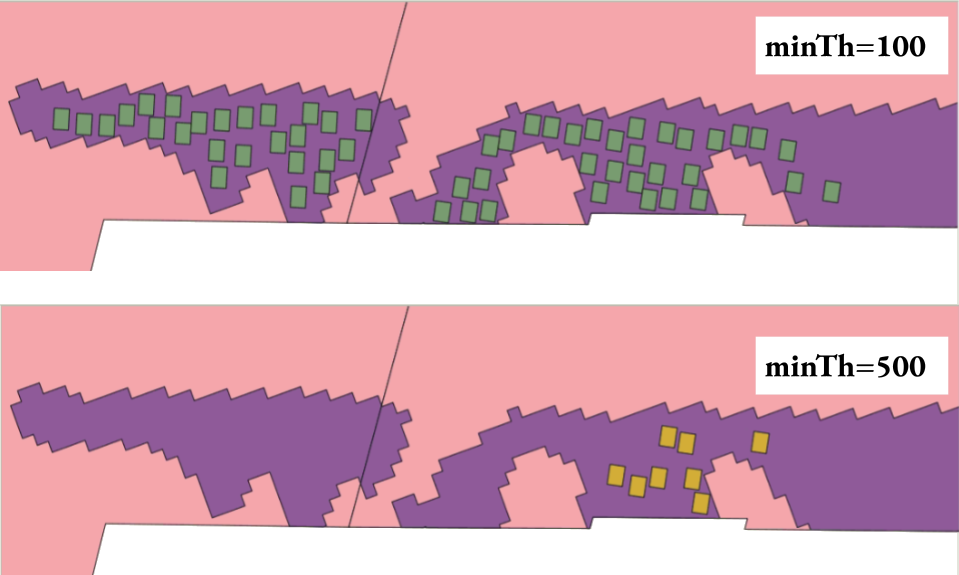
\includegraphics[width=0.9\linewidth]{images/100vs500.png}\vspace{-0.4cm}
\caption{{Result of the placement algorithm on a small portion of the district (i.e., two roofs) with threshold $minTh=100$ (top) and $minTh=500$ (bottom): the pink area represents the area of the roofs, the purple area is the suitable area, and the rectangles represent PV modules placed on locations with 75th percentile higher than $minTh$. As expected, the second placement contains less PV modules, as the minimum threshold is set to a higher value. }}
\label{fig:satellizeZoom}
\end{figure}

\subsection{Energy production performance}
To analyze the performance of the algorithm in terms of power outcome, we compared the yearly production of the identified optimal placements w.r.t. a traditional placement of the same number of PV modules. The traditional placement is built by positioning PV modules in a more standard positioning (i.e., a \virgolette{compact} rectangular placement that does not consider the 75th percentile of irradiance).
% them in the suitable area but with a more standard positioning (i.e., a \virgolette{compact} rectangular placement that does not consider the 75th percentile of irradiance), built by the algorithm proposed in \cite{soarespredicting}. Consider that the traditional placement is positioned in the suitable area and thus benefits from the preliminary analysis of irradiance and of shadow distribution, thus being a competitive placement.  
%To analyze the performance we compared the result of the energy production for the configurations obtained with our algorithm with classical configurations with the same amount of panels. The classical configurations were obtained with a custom implementation of the algorithm described in \cite{soarespredicting} that did not take into account the limitation imposed by the threshold on the irradiance. 

Table \ref{tab:production} shows that the production of the optimal PV installations is always larger than the one of the corresponding traditional placement, and as expected the production of the different configuration decreases linearly with the number of panels installed. However, it is interesting to notice that the improvement of power production is higher with higher values of $minTh$, with maximum improvement of 21\% with threshold 500 (as shown in the Table and reported in the third plot of Figure \ref{fig:production}). This behaviour can be easily explained by considering that the lower the threshold the higher the number of PV panels, and thus of potential overlap of positions of PV modules for the two placements. Vice versa, with higher thresholds the number of PV modules is reduced and the optimal placement can succesfully select only the positions less affected by shading. This reduces the impact of the bottleneck effect of partial shading on the output power production of the optimal PV placement. This analysis is confirmed by the amound of area shared by the two placements, that is higher with $minTh=100$ (36\%) and decreases with higher values of $minTh$, with a minumum of 15\% with $minTh=500$.  
% is due to the fact that having an high threshold for the 75-percentile of the irradiance allow the algorithm to use only the best positions for the panel thus reducing the impact of shading and the bottleneck effect that is normally caused by the least irradiated PV modules.%from the result summarized in the Table \ref{tab:production} and shown in plot 3 of Figure \ref{fig:production} that the optimal placement bring better result w.r.t. the classical placement when the number of panels is lower with up to a 21\% of improvement in the performance when the threshold is at 500. This behaviour is due to the fact that having an high threshold for the 75-percentile of the irradiance allow the algorithm to use only the best positions for the panel thus reducing the impact of shading and the bottleneck effect that is normally caused by the least irradiated PV modules.

% \begin{table}[!tbp]
% \centering
% %\resizebox{\linewidth}{!}{%
% %\begin{tabular}{|p{1.5cm}|p{1.5cm}|p{1.5cm}|p{1.5cm}|p{1.5cm}|}
% %\hline
% %\textbf{75-th percentile threshold} &\textbf{N of panels}&\textbf{Classic \newline configuration $P_{yearly}$(MW)}  & \textbf{Optimal \newline  configuration $P_{yearly}$(MW)} &\textbf{Improvement of optimal vs. classic} \\

% \begin{tabular}{|r|r|r|r|r|}
% \hline
% \textbf{Threshold} & \textbf{Panels} & \multicolumn{2}{c|}{\textbf{Power production (MW)}} & \textbf{Improvement}\\
% \cline{3-4}
% \textbf{($minTh$)} & \multicolumn{1}{c|}{\textbf{(\#)}} & \textbf{Optimal} & \multicolumn{1}{c|}{\textbf{Traditional}} & \multicolumn{1}{c|}{\textbf{(\%)}}\\
% \hline\hline
% 100 & 1,792 & 1,015 & 998 & 1.6\% \\\hline
% 200 & 1,536 & 905 & 874 & 3.6\% \\\hline
% 300 & 656 & 423 & 376 & 12.6\% \\\hline
% 400 & 464 & 323 & 277 & 16.9\% \\\hline
% 500 & 176 & 139 & 115 & 20.8\% \\\hline
% \end{tabular}%
% \caption{Summary of the comparison among the optimal placement with varying $minTh$ w.r.t. a traditional placement of the same number of panels \attenzione{è possibile stimare se c'è un overlap tra i due placement, i.e., quanti pannelli sono nella stessa posizione?}}
% \label{tab:production}
% \end{table}


%\resizebox{\linewidth}{!}{%
%\begin{tabular}{|p{1.5cm}|p{1.5cm}|p{1.5cm}|p{1.5cm}|p{1.5cm}|}
%\hline
%\textbf{75-th percentile threshold} &\textbf{N of panels}&\textbf{Classic \newline configuration $P_{yearly}$(MW)}  & \textbf{Optimal \newline  configuration $P_{yearly}$(MW)} &\textbf{Improvement of optimal vs. classic} \\
\begin{table}[!tbp]
\centering
\caption{Summary of the comparison among the optimal placement with varying $minTh$ w.r.t. a traditional placement of the same number of panels.}
\label{tab:production}
\begin{tabular}{|r|r|r|r|r|r|}
\hline
\textbf{Threshold} & \textbf{Panels} &\textbf{Shared} & \multicolumn{3}{c|}{\textbf{Power production (MW)}} \\
\cline{4-6}
\textbf{($minTh$)} & \multicolumn{1}{c|}{\textbf{(\#)}} & \multicolumn{1}{c|}{\textbf{area (\%)}}& \textbf{Optimal} & \multicolumn{1}{c|}{\textbf{Traditional}} & \multicolumn{1}{c|}{\textbf{(\%)}}\\
\hline\hline
100 & 1,792 &36 & 1,015 & 998 & +1.6\% \\\hline
200 & 1,536 &31 & 905 & 874 & +3.6\% \\\hline
300 & 656 &22 & 423 & 376 & +12.6\% \\\hline
400 & 464 &23 & 323 & 277 & +16.9\% \\\hline
500 & 176 &15 & 139 & 115 & +20.8\% \\\hline
\end{tabular}%
\end{table}

\begin{figure}[!tbp]
\centering
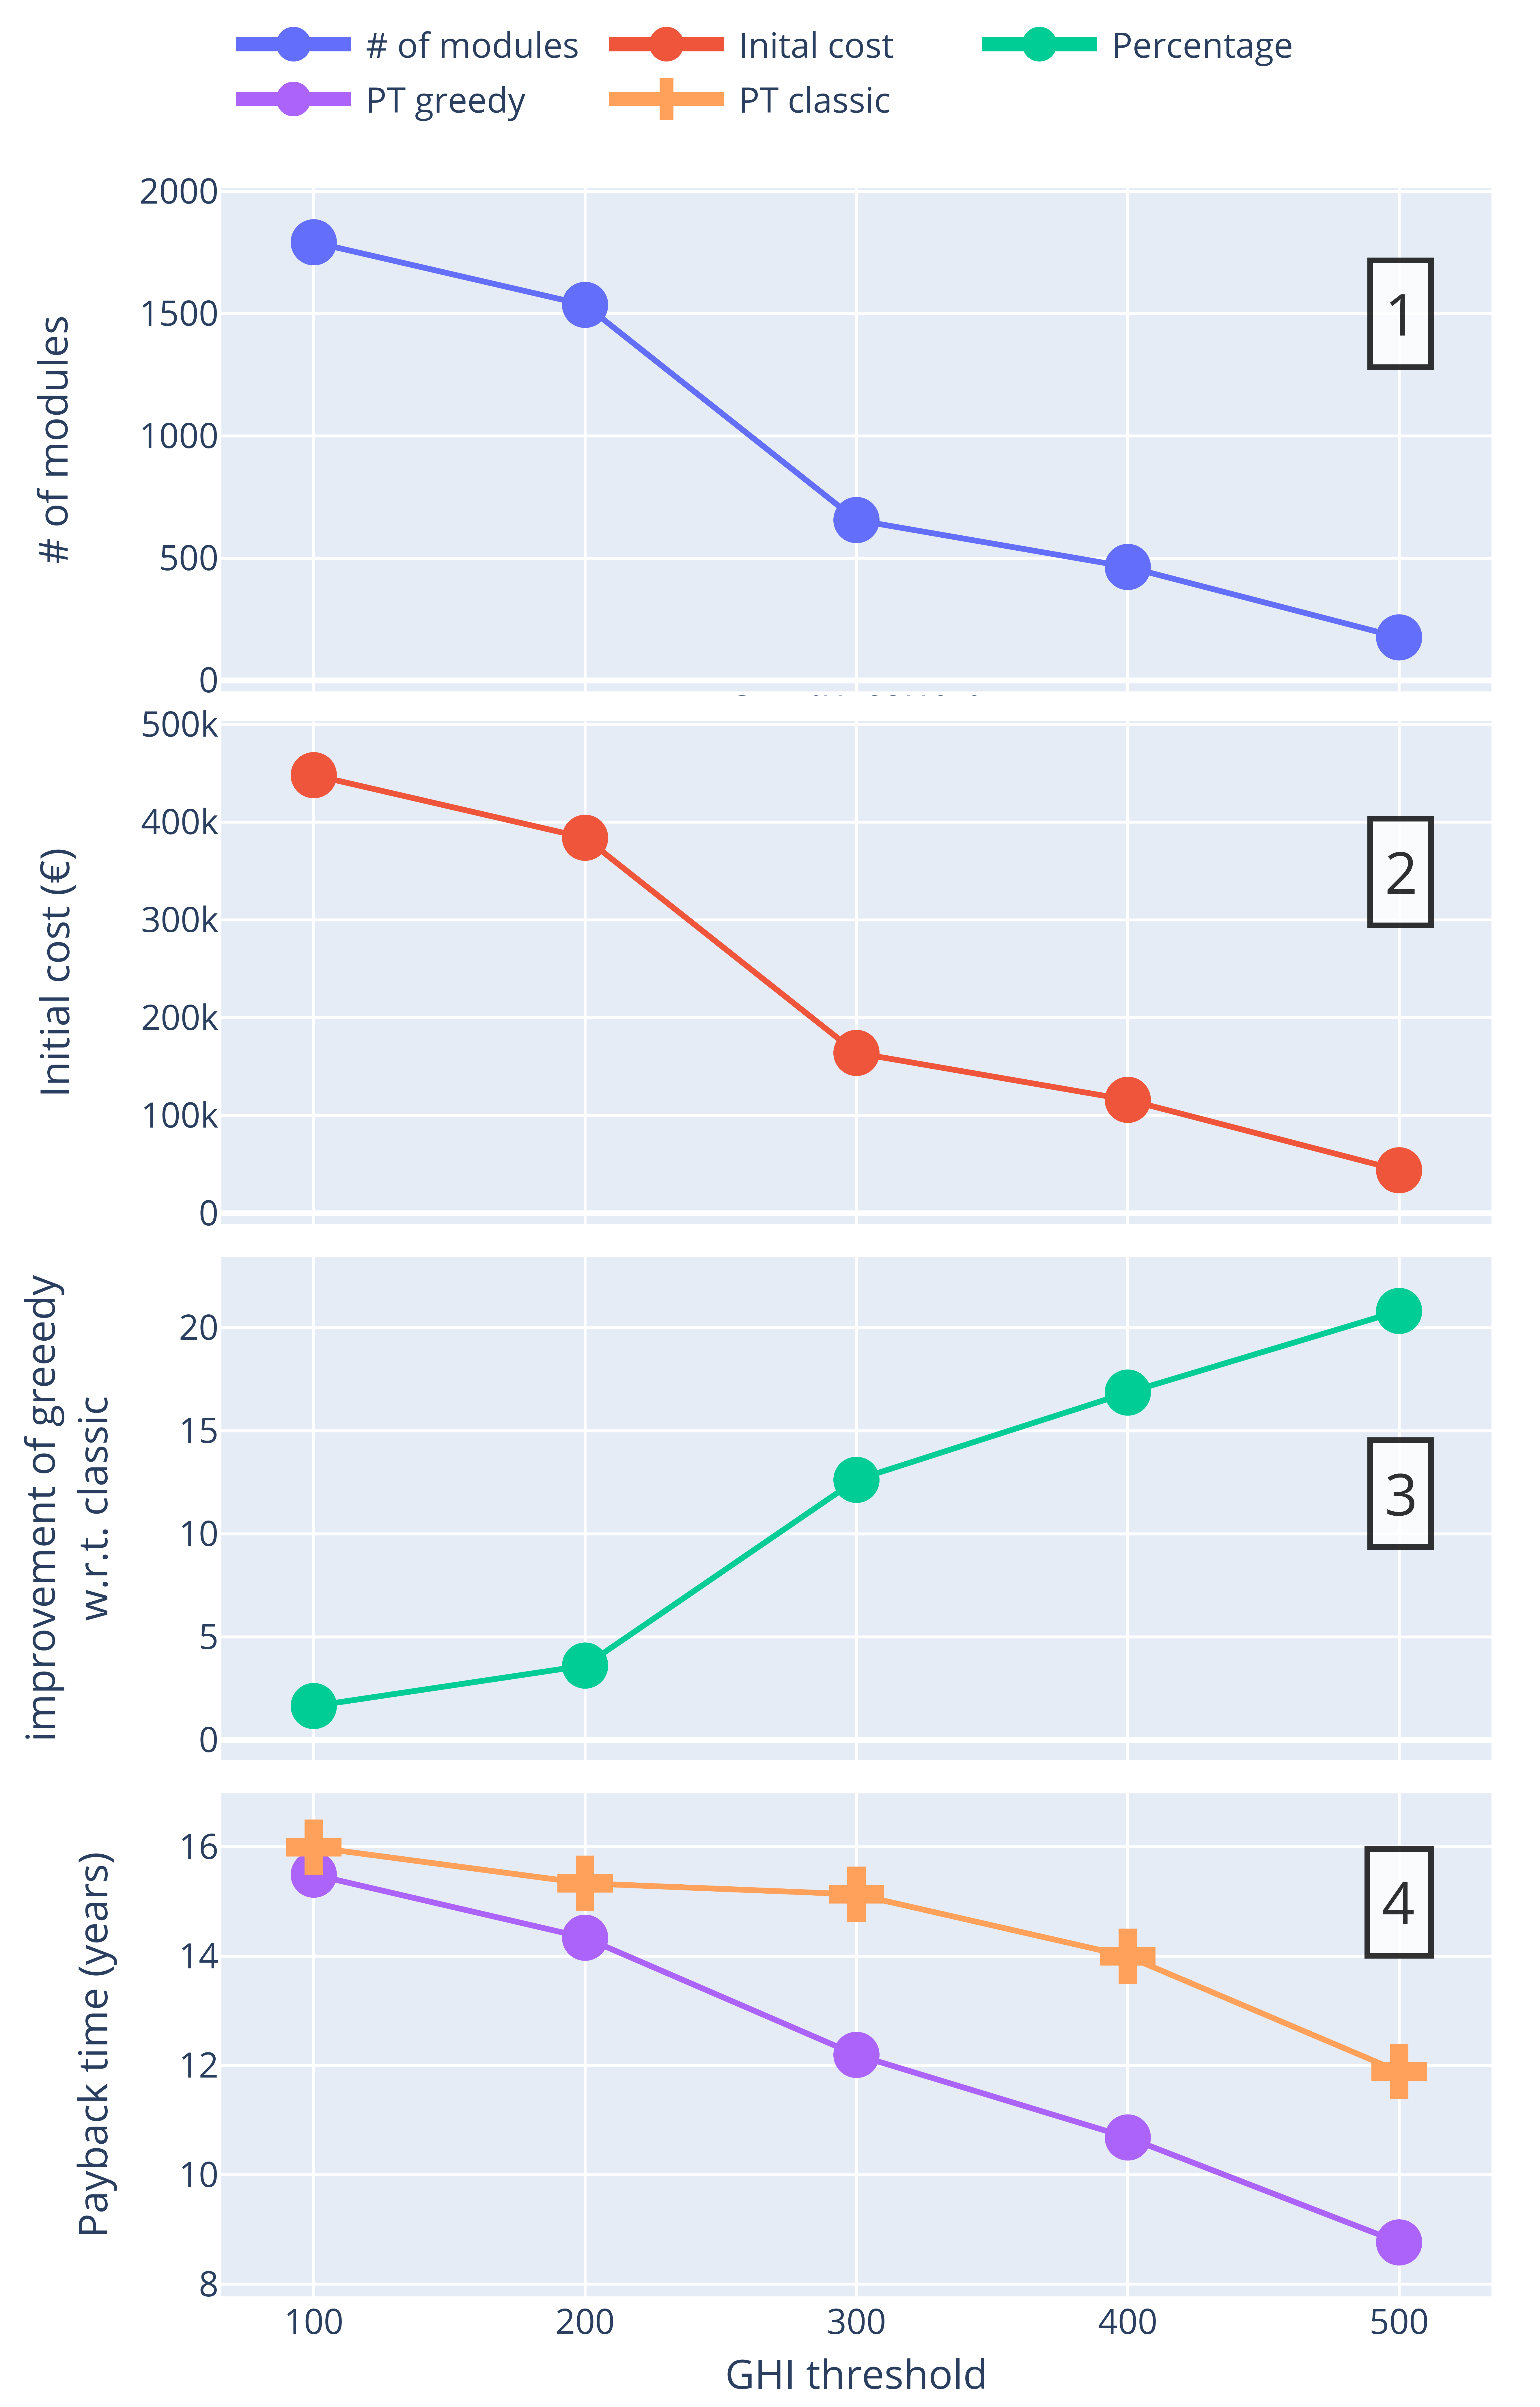
\includegraphics[width=\linewidth]{images/stacked_annotated2.png}\vspace{-0.4cm}
\caption{Behavior of the placement algorithm with different values of $minTh$: number of PV modules (1), initial installation cost (2), improvement of power production w.r.t. the traditional placement (3), payback time (4) (orange for the proposed algorithm, purple for the traditional placement).}
\label{fig:production}
\end{figure}
\subsection{Payback time}
Using the procedure explained in \ref{sec:economic} we evaluated the PT for both the classic and the optimal configuration considering also the different value of the threshold. The energy price considered is 0.22€ per kWh \cite{energy_price}, the panel cost is 250€ per panel and the maintenance cost considered is 15€ per panel per year. The plot 4 in Figure \ref{fig:production} shows how the PT decreases together with the number of panels and that the payback times of the PV installation produced by our framework are always lower than the classical ones. In particular when the threshold is at 500 the configuration produced by the framework reduces by $1/4$ the PT. However by comparing the result in \ref{tab:production} and the Figure \ref{fig:production} we can notice while increasing the amount of panels increases the production and therefore the earning this does not decrease the PT that instead increases. This underlines how this kind of analysis are useful for an EA that needs to take into account this economic analysis to plan his investment.


% correggere reference al grafico, aggiungere unita di misura all'asse y e nome asse x con descrizione, scrivere meglio didascalia figura, aggiungere numero ai grafici per citarli nel testo

